\documentclass[11pt]{article}
\renewcommand{\baselinestretch}{1.05}
\usepackage{amsmath,amsthm,verbatim,amssymb,amsfonts,amscd, graphicx}
\usepackage{blindtext}

\usepackage{caption}
\usepackage{enumitem}

%Additional Packages
\usepackage{enumitem}
\usepackage{graphics}
\usepackage{float}
\graphicspath{ {images/} }
%\usepackage[framed]{mcode}
\usepackage{hyperref}
\hypersetup{
	colorlinks=true,
	linkcolor=blue,
	filecolor=magenta,      
	urlcolor=cyan,
}

\topmargin0.0cm
\headheight0.0cm
\headsep0.0cm
\oddsidemargin0.0cm
\textheight23.0cm
\textwidth16.5cm
\footskip1.0cm
\theoremstyle{plain}
\newtheorem{theorem}{Theorem}
\newtheorem{corollary}{Corollary}
\newtheorem{lemma}{Lemma}
\newtheorem{proposition}{Proposition}
\newtheorem*{surfacecor}{Corollary 1}
\newtheorem{conjecture}{Conjecture} 
\newtheorem{question}{Question} 
\theoremstyle{definition}
\newtheorem{definition}{Definition}

\usepackage{indentfirst}
%\renewcommand{\thesubsubsection}{\thesubsection.\alph{subsection}}

\newcommand{\floor}[1]{\lfloor #1 \rfloor}

%SETUP PSUEDOCODE
\usepackage{tcolorbox}


%SETUP AtxMEGA128A1U
\usepackage{listings}

\usepackage{xcolor}
\definecolor{bluekeywords}{rgb}{0.13,0.13,1}
\definecolor{greencomments}{rgb}{0,0.5,0}
\definecolor{turqusnumbers}{rgb}{0.17,0.57,0.69}
\definecolor{redstrings}{rgb}{0.5,0,0}


%Set up code
\usepackage{listings}
\usepackage{color}

\definecolor{dkgreen}{rgb}{0,0.6,0}
\definecolor{gray}{rgb}{0.5,0.5,0.5}
\definecolor{mauve}{rgb}{0.58,0,0.82}

\lstset{frame=tb,
	language=C,
	aboveskip=3mm,
	belowskip=3mm,
	showstringspaces=true,
	columns=flexible,
	basicstyle={\small\ttfamily},
	numbers=none,
	numberstyle=\tiny\color{gray},
	keywordstyle=\color{blue},
	commentstyle=\color{dkgreen},
	stringstyle=\color{mauve},
	breaklines=true,
	breakatwhitespace=true,
	tabsize=3
}

%
% START OF DOCUMENT
%
\begin{document}
\captionsetup[figure]{labelfont=bf} 

\title{Lab 7}
\author{\textbf{Michael}\\Lab Section: 7F34}
\maketitle
%
% PRELAB QUESTIONS
%
\section*{b. Answers to all pre-lab questions}



\begin{enumerate}[label={\arabic*)},font={\color{red}\bfseries}]
	%
	%1
	%
	\item If the NAD/DAD board were not available, nor any conventional desktop measuring tools (like a voltmeter), how could you verify that your DAC were functioning properly
	\\[0.8ex]
	\textbf{ANS: } One way to check is to use ADC(analog to digital converter) to verify.  The DAC output would be sent to a ACD input, then using conversions and usart (LAB 5), the values can be outputted to a terminal. 
	%
	%2
	%
	\item You probably noticed that your sine wave does not look very good. While at least meeting specifications, how could you increase the quality of your sine wave?
	\\[0.8ex]
	\textbf{ANS: } To increase the quality of my sine wave, 2 things must be done. The first is that more data points would have to be used. The second thing is the timer would have to be decreased (the PER) in order to keep the desired Hz
	%
	%3
	%
	\item How many DMA channels are available on the XMEGA?
	\\[0.8ex]
	\textbf{ANS: } CH0, CH1, CH2, and CH3 are available for a total of 4 DMA channels on the XMEGA. 
	%
	%4
	%
	\item How many different options are there to trigger the DMA?
	\\[0.8ex]
	\textbf{ANS: } There are 26 different options to trigger the DMA.
	%
	%5
	%
	\item While you were not asked to implement this in your lab, explain how one might vary the amplitude of an output wave, much like the frequency was varied. 
	\\[0.8ex]
	\textbf{ANS: } One might change the amplitude of the output wave by using a reference higher than the one currently used (not using AREFB). Then one would have to increase/add values in the sine table higher than 0xFFF.
\end{enumerate}
%
% PROBLEMS ENCOUNTERED
%
\section*{c. Problems Encountered} 
Problems encounter was that in part D, the wave type would not switch if the output was set to 0. This was fixed by resetting the DMA every time it was switched
%
% FUTURE WORK
%
\section*{d. Future Work/Applications}
Future application would be using the speaker. Instead of using data for a sine wave, the data can be for musical notes and the notes can be played from the speaker.
%
% SCHEMATICS
%
\section*{e. Schematics}
N/A
%
% PSEUDOCODE
%
\newpage
\section*{g. Pseudocode/Flowcharts}
%
% PSEUDOCODE PART A
%
\textbf{\textcolor{blue}{Pseudocode for Lab7A.c:}}
\begin{tcolorbox}
\begin{verbatim}
MAIN:
    * Call Change_CLK_32HZ Function
    * Call DAC_INIT();
    * Output 1.3V
    
    WHILE(TRUE);
END  

FUNCTION DAC_INIT 
    * Set up port A
    * Set up DAC controls
    
FUNCTION UPDATE_DACA_CH0
    * Update DACA.CH0 data
        
FUNCTION Change_CLK_32HZ
    * Enable the new oscillator

    WHILE(OSC FLAG not set){}

    * Write the “IOREG” signature to the CPU_CCP reg
    * Select the new clock source in the CLK_CTRL reg  
\end{verbatim}
\end{tcolorbox}
%
% PSEUDOCODE PART B
%
\newpage
\textbf{\textcolor{blue}{Pseudocode for Lab7B.c:}}
\begin{tcolorbox}
\begin{verbatim}
MAIN:
    * Call Change_CLK_32HZ Function
    * Call DAC_INIT
    * Call COUNTER_INIT
    * Call COUNTER_START
    
    * Enable interrupts
    
    WHILE(TRUE);
END  

FUNCTION COUNTER_INIT
    * Set top of counter

FUNCTION COUNTER_START
    * Set interupt for counter
    * Start COUNTER
    
ISR TCC0_OVF_vect
    * Preserve Status Reg     
    * Change output 
    IF(COUNTER equals 100){
        * Reset Counter
    }
    * Clear interrupt flags
    * Restore Status Reg
    
FUNCTION DAC_INIT 
    * Set up port A
    * Set up DAC controls
	
FUNCTION UPDATE_DACA_CH0
    * Update DACA.CH0 data
	
FUNCTION Change_CLK_32HZ
    * Enable the new oscillator
	
    WHILE(OSC FLAG not set){}
	
    * Write the “IOREG” signature to the CPU_CCP reg
    * Select the new clock source in the CLK_CTRL reg  
\end{verbatim}
\end{tcolorbox}
%
% PSEUDOCODE PART C
%
\newpage
\textbf{\textcolor{blue}{Pseudocode for Lab7C.c:}}
\begin{tcolorbox}
\begin{verbatim}
    MAIN:
    * Call Change_CLK_32HZ Function
    * Call DAC_INIT
    * Call DMA_INIT
    * Call COUNTER_INIT
    * Call COUNTER_START
	
    * Enable interrupts
	
    WHILE(TRUE);
END  
	
	
FUNCTION DMA_INIT
    * Enable DMA
    * Set up ADDRESS CONTROL
    * Set up TRIGGER SOURCE
    * Set up CH BLOCK TRANSFER COUNT
    * Set up DMA as CONTINOUS
    * Set up Source Address
    * Set up Destination Address
    * Set up CH0 control 
    	
	
FUNCTION COUNTER_INIT
    * Set top of counter

FUNCTION COUNTER_START
    * Set interupt for counter
    * Start COUNTER
	
ISR TCC0_OVF_vect
    * Preserve Status Reg
    * Clear interrupt flags
    * Restore Status Reg
	
FUNCTION DAC_INIT 
    * Set up port A
    * Set up DAC controls
	
FUNCTION UPDATE_DACA_CH0
    * Update DACA.CH0 data
\end{verbatim}
\end{tcolorbox}
\begin{tcolorbox}
\begin{verbatim}
FUNCTION Change_CLK_32HZ
    * Enable the new oscillator
	
    WHILE(OSC FLAG not set){}
	
    * Write the “IOREG” signature to the CPU_CCP reg
    * Select the new clock source in the CLK_CTRL reg  
\end{verbatim}
\end{tcolorbox}
%
% PSEUDOCODE PART D
%
\newpage
\textbf{\textcolor{blue}{Pseudocode for Lab7D.c:}}
\begin{tcolorbox}
\begin{verbatim}
    MAIN:
    * Call Change_CLK_32HZ Function
    * Call DAC_INIT
    * Call DMA_INIT
    * Call COUNTER_INIT
    * Call COUNTER_START
    * Call USART_INIT
    * Enable interrupts
    WHILE(TRUE){
        * Display Menu
        * Get User input
    	SWITCH(user input){
    	    CASE 's' CASE 'S'
    	        * Change DMA with Sine data
    	    CASE 't' CASE 'T'
    	        * Change DMA with Triangle data
    	    CASE '0'
    	        * Turn off TCC0
    	        * Output 0v
    	    CASE '1'
    	        * Change Hz to 50*1
    	    CASE '2'
    	        * Change Hz to 50*2
    	    CASE '3'
    	        * Change Hz to 50*3
    	    CASE '4'
    	        * Change Hz to 50*4
    	    CASE '5'
    	        * Change Hz to 50*5
    	    CASE '6'
    	        * Change Hz to 50*6
    	    CASE '7'
    	        * Change Hz to 50*7
    	    CASE '8'
    	        * Change Hz to 50*8
    	    CASE '9'	
    	        * Change Hz to 50*9    
    	}
    	IF(choice is 1 - 9){
    	    * Call COUNTER_START()
    	}
    } 
END  
\end{verbatim}
\end{tcolorbox}
\begin{tcolorbox}
\begin{verbatim}
FUNCTION DISPLAY_MENU
    * Make Menu Strings
    * Set up array of menu strings	
    FOR(int i = 0; i < size; i++){
        * Display string
    }
    
FUNCTION USART_INIT
    * Set port D for USART com
    * Set up Ctrl B and C
    * Set up baud rate

FUNCTION OUT_STRING
    While(char[] does not equal NULL){
        * Call OUT_CHAR
    }

FUNCTION OUT_CHAR
    While(Transmitting){}
    * Return USART Data in a CHAR    

FUNCTION IN_CHAR
    * WHILE(Recieving){}
    * Return data 
	
FUNCTION DMA_INIT
    * Enable DMA
    * Set up ADDRESS CONTROL
    * Set up TRIGGER SOURCE
    * Set up CH BLOCK TRANSFER COUNT
    * Set up DMA as CONTINOUS
    IF(MODE is SINE){
        * Call SINE_SOURCE_DES
    }
    ELSE IF(MODEis TRIANGLE){
       * Call TRIANGLE_SOURCE_DES
    }
    * Set up CH0 control 
    
FUNCTION SINE_SOURCE_DES   
    * Wait until CH is not busy
    * Set up address with Sine
    * Set up Source Address
    * Set up Destination Address
\end{verbatim}
\end{tcolorbox}
\begin{tcolorbox}
\begin{verbatim}    
FUNCTION TRIANGLE_SOURCE_DES
    * Wait until CH is not busy
    * Set up address with Sine
    * Set up Source Address
    * Set up Destination Address	
	
FUNCTION COUNTER_INIT
    * Set top of counter
	
FUNCTION COUNTER_START
    * Set interupt for counter
    * Start COUNTER
	
ISR TCC0_OVF_vect
    * Preserve Status Reg
    * Clear interrupt flags
    * Restore Status Reg
	
FUNCTION DAC_INIT 
    * Set up port A
    * Set up DAC controls
	
FUNCTION UPDATE_DACA_CH0
    * Update DACA.CH0 data
	
FUNCTION Change_CLK_32HZ
    * Enable the new oscillator
	
    WHILE(OSC FLAG not set){}
	
    * Write the “IOREG” signature to the CPU_CCP reg
    * Select the new clock source in the CLK_CTRL reg  
\end{verbatim}
\end{tcolorbox}
\newpage
%
%
% PROGRAM CODE
%
%
\section*{h. Program Code}
\textbf{\textcolor{blue}{Code for Lab7A.c:}}
\lstinputlisting{Lab7A.c}
\newpage
\textbf{\textcolor{blue}{Code for Lab7B.c:}}
\lstinputlisting{Lab7B.c}\
\newpage
\textbf{\textcolor{blue}{Code for Lab7C.c:}}
\lstinputlisting{Lab7C.c}
\newpage
\textbf{\textcolor{blue}{Code for Lab7D.c}}
\lstinputlisting{Lab7D.c}
\newpage
%
%
% APPENDIX
%
%
\section*{i. Appendix}
\begin{figure}[H]
	\centering
	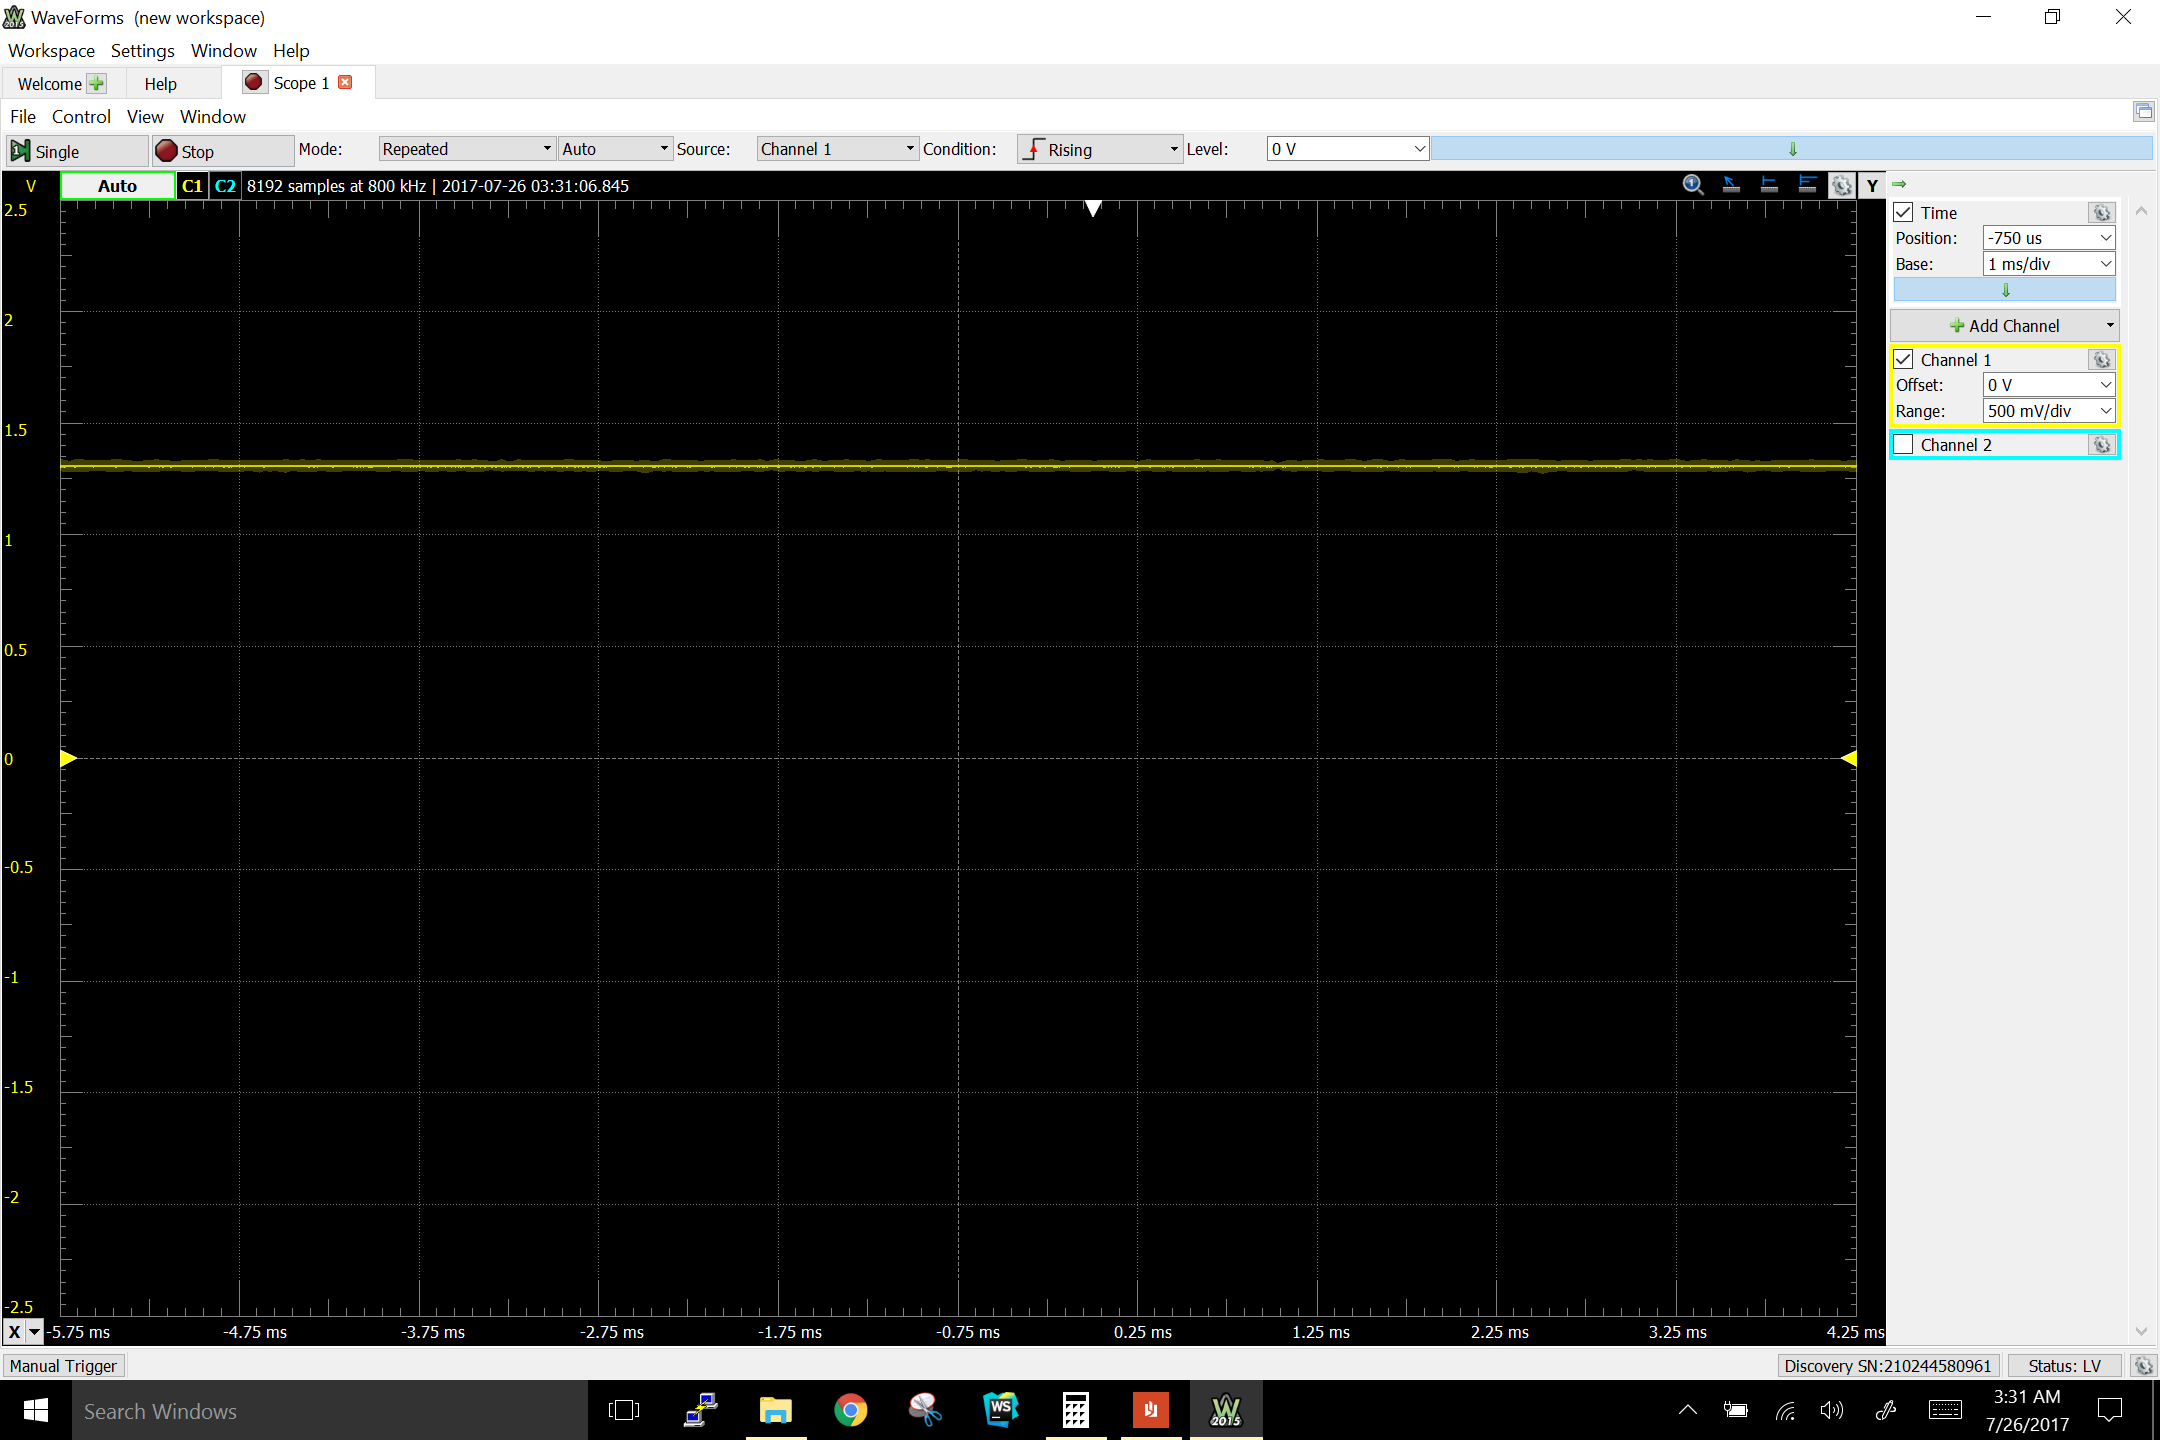
\includegraphics[width=\textwidth]{A}
	\label{fig:a}
	\caption{DAD reading of constant 1.3V signal}
\end{figure}
\begin{figure}[H]
	\centering
	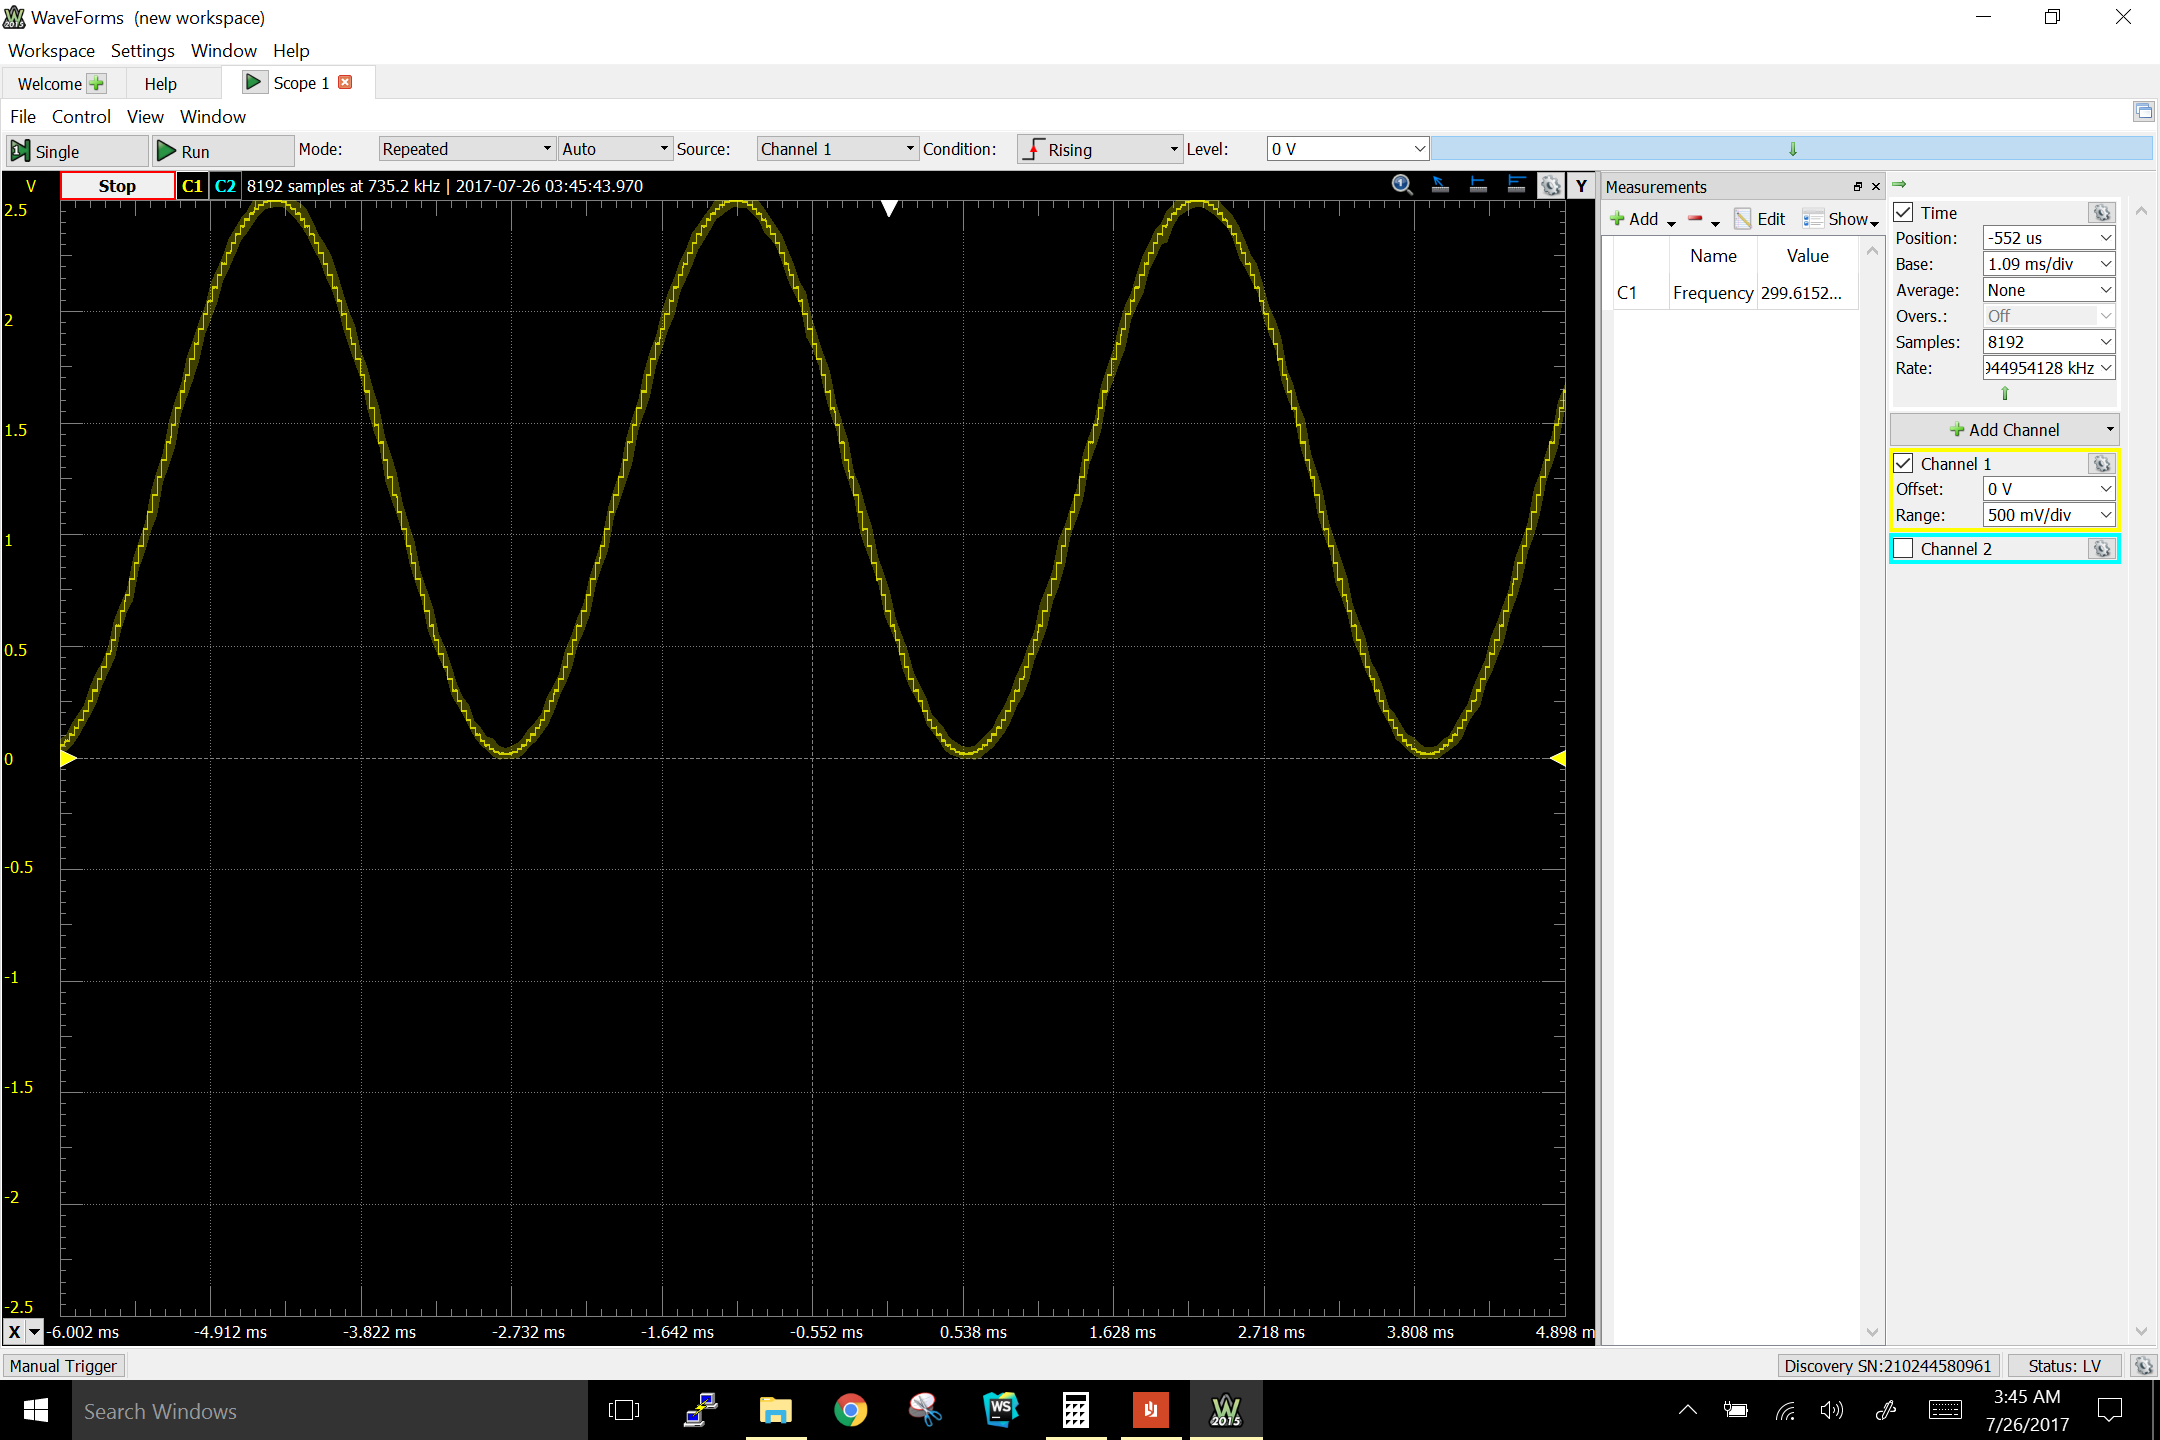
\includegraphics[width=\textwidth]{B}
	\label{fig:b}
	\caption{300Hz sine wave}
\end{figure}
\begin{figure}[H]
	\centering
	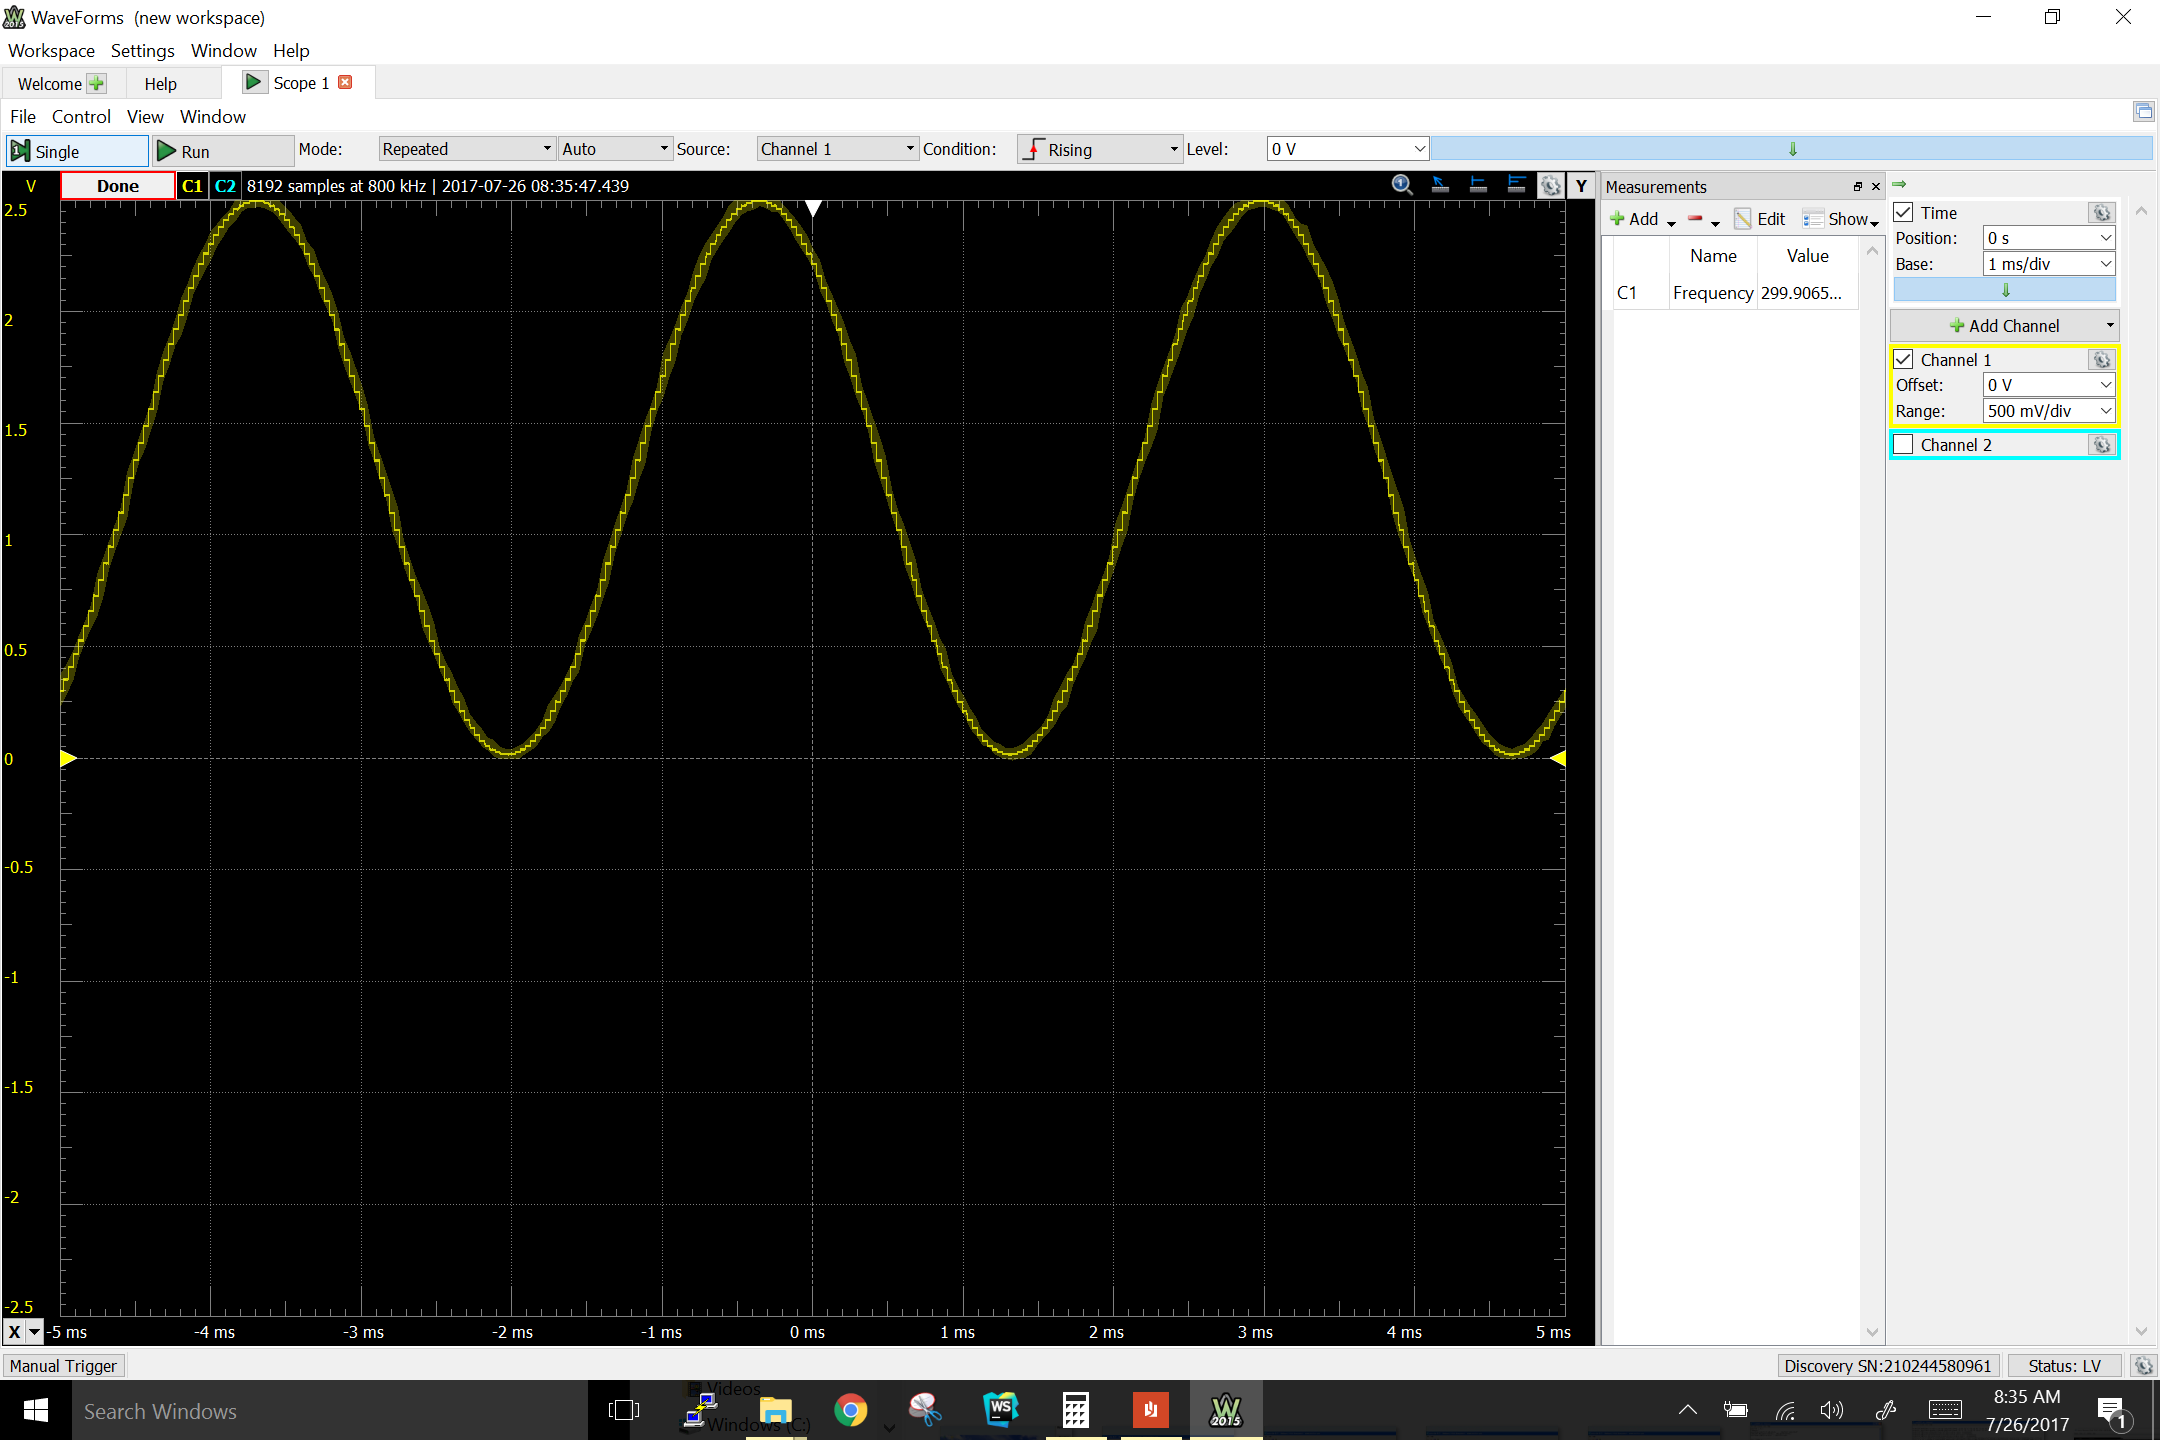
\includegraphics[width=\textwidth]{C}
	\label{fig:c}
	\caption{300Hz sine wave (with DMA)}
\end{figure}
\begin{figure}[H]
	\centering
	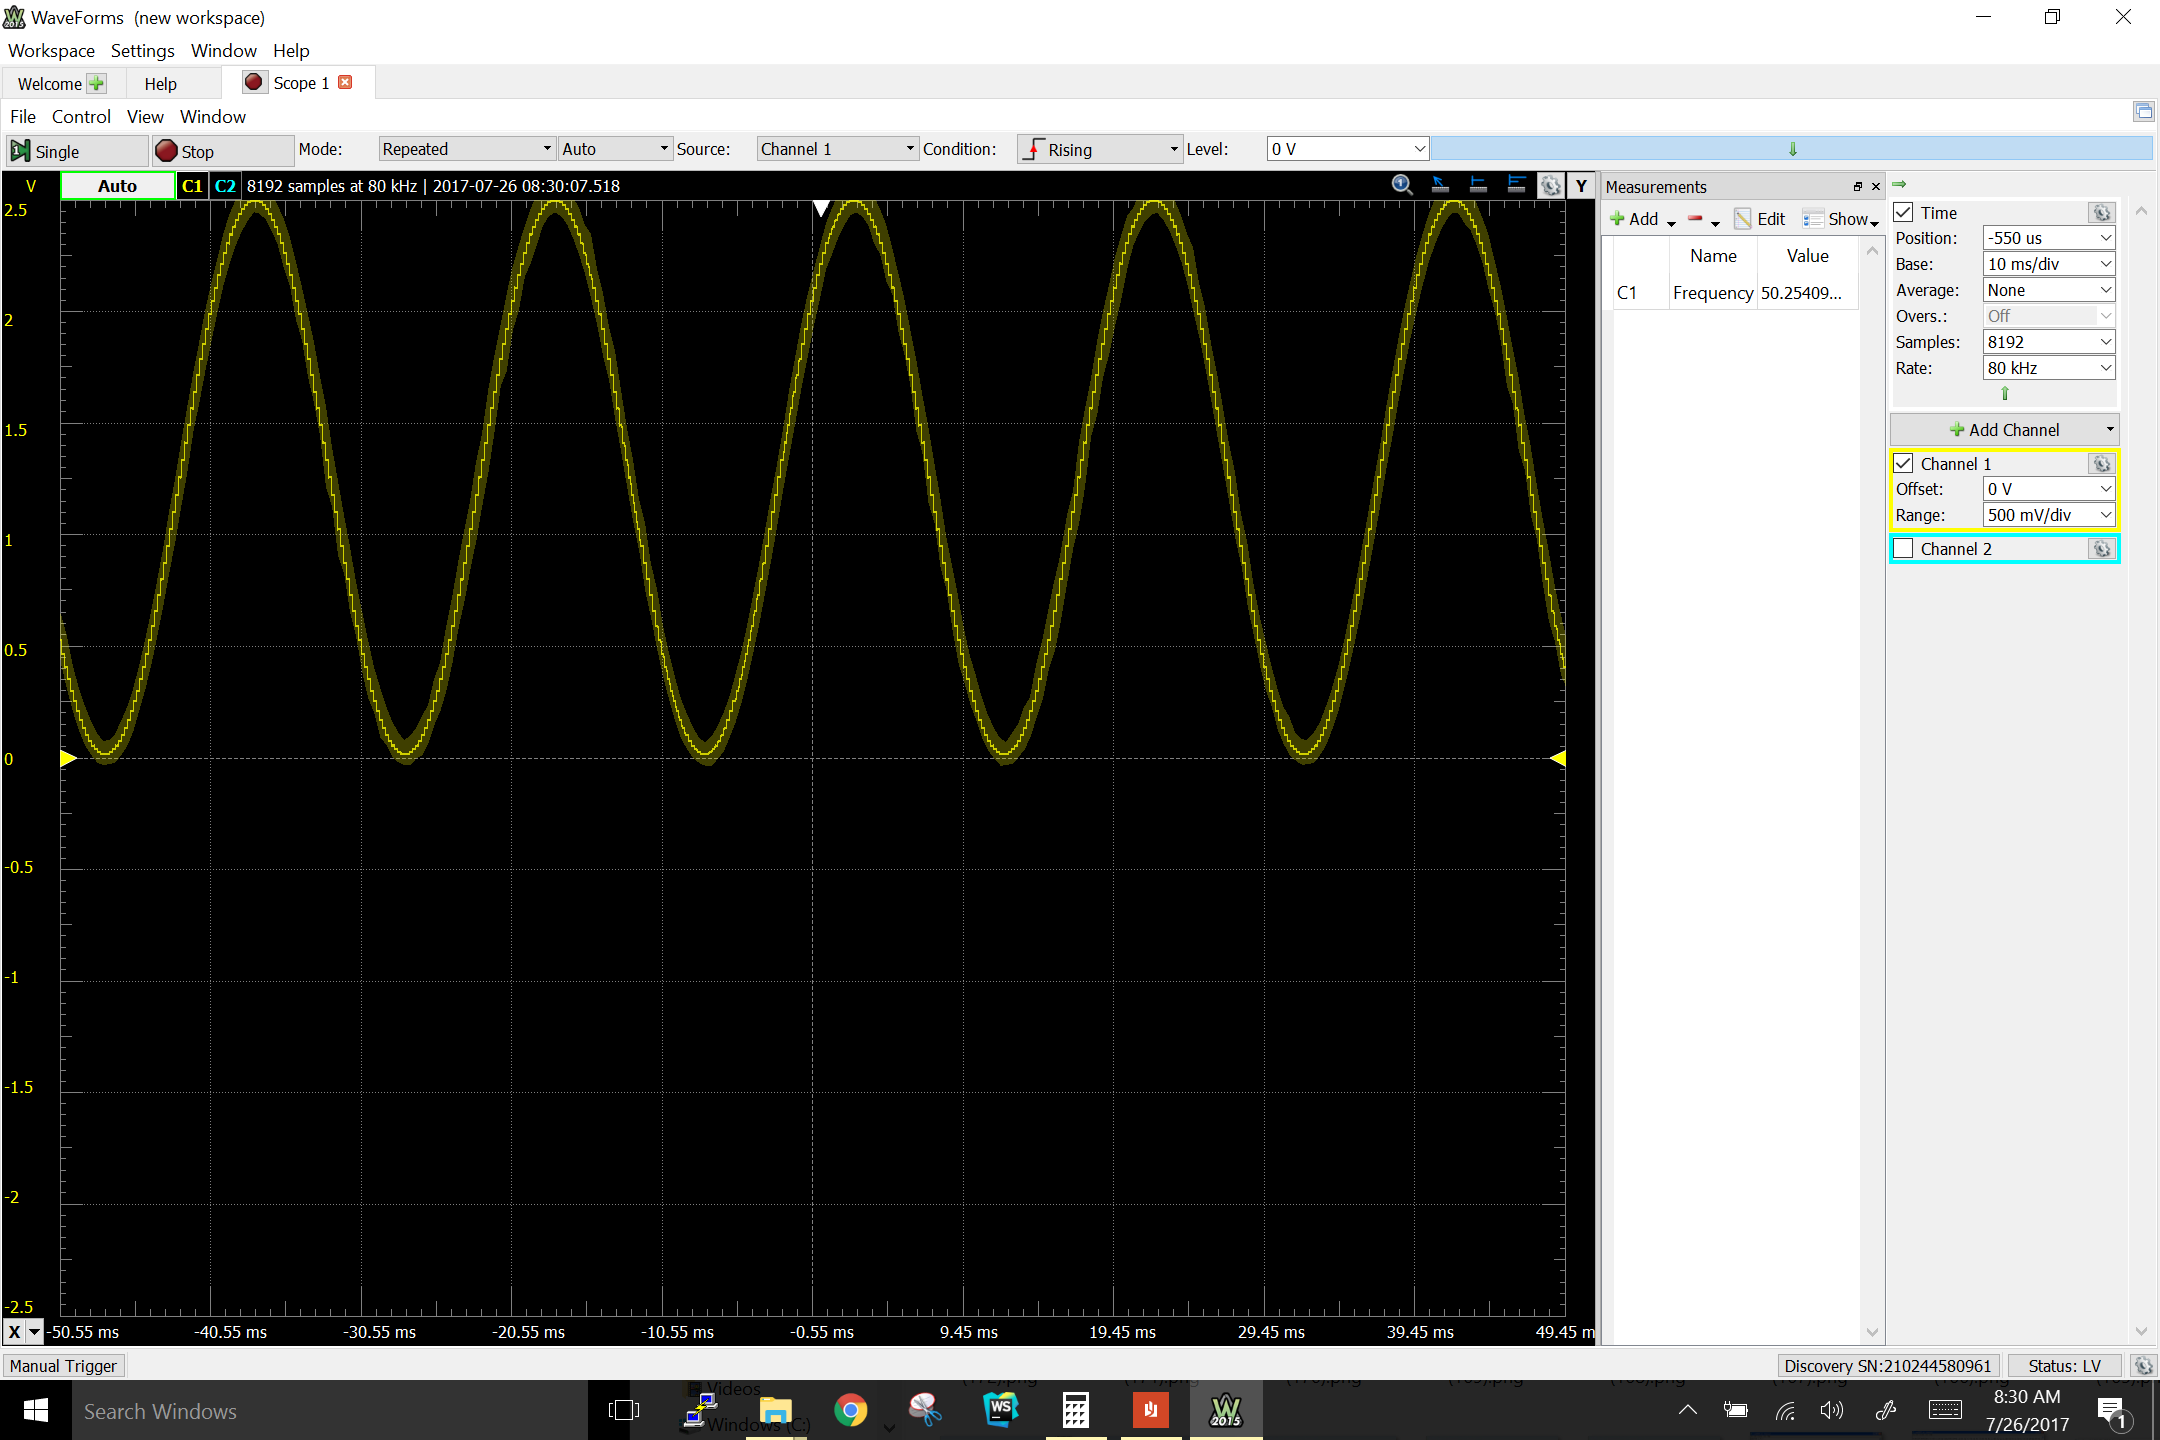
\includegraphics[width=\textwidth]{D1}
	\label{fig:c}
	\caption{50Hz sine wave}
\end{figure}
\begin{figure}[H]
	\centering
	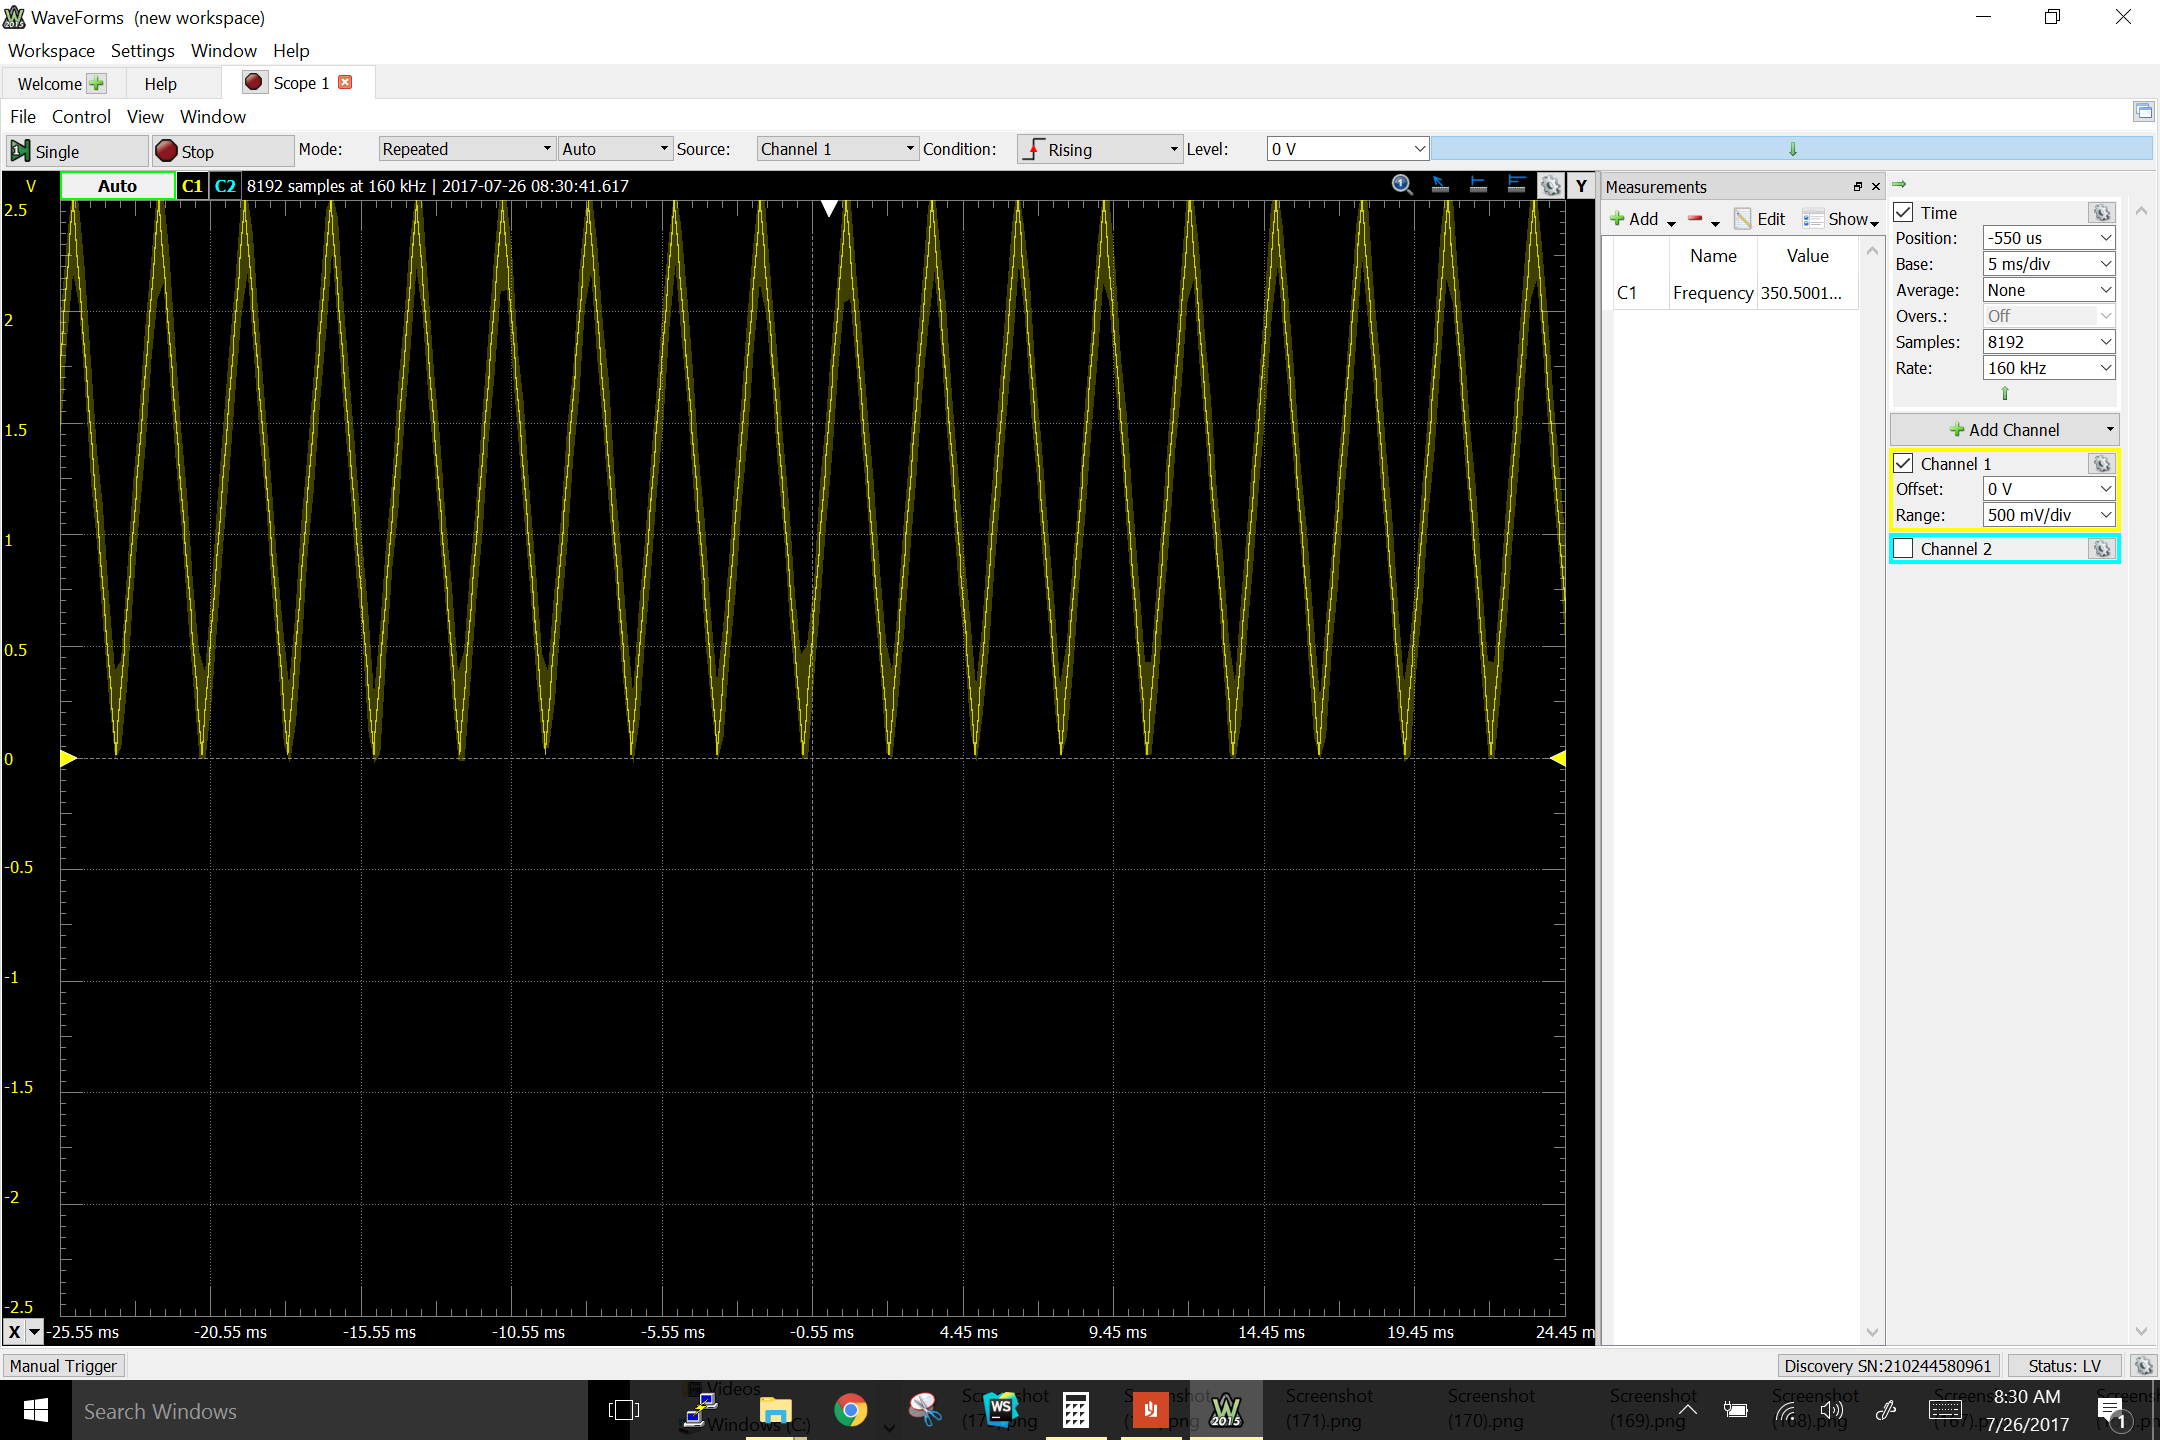
\includegraphics[width=\textwidth]{D2}
	\label{fig:c}
	\caption{350Hz triangle wave}
\end{figure}
%
% HEADER FILES
%
\newpage
%
% Clk_32Mhz
%
\textbf{\textcolor{blue}{Code for Clk\textunderscore 32MHz.h:}}
\lstinputlisting{Clk_32MHz.h}
\newpage
\textbf{\textcolor{blue}{Code for Clk\textunderscore 32MHz.c:}}
\lstinputlisting{Clk_32MHz.c}
%
% DAC
%
\newpage
\textbf{\textcolor{blue}{Code for DAC.h:}}
\lstinputlisting{DAC.h}
\newpage
\textbf{\textcolor{blue}{Code for DAC.c:}}
\lstinputlisting{DAC.c}
%
% DMA
%
\newpage
\textbf{\textcolor{blue}{Code for DMA.h:}}
\lstinputlisting{DMA.h}
\newpage
\textbf{\textcolor{blue}{Code for DMA.c:}}
\lstinputlisting{DMA.c}
%
% TIMER_COUNTER
%
\newpage
\textbf{\textcolor{blue}{Code for TIMER\textunderscore COUNTER.h:}}
\lstinputlisting{TIMER_COUNTER.h}
\newpage
\textbf{\textcolor{blue}{Code for TIMER\textunderscore COUNTER.c:}}
\lstinputlisting{TIMER_COUNTER.c}
\newpage
\textbf{\textcolor{blue}{Code for TIMER\textunderscore COUNTER.c (Part B):}}
\lstinputlisting{TIMER_COUNTER_B.c}
%
% USART 
%
\newpage
\textbf{\textcolor{blue}{Code for USART.h:}}
\lstinputlisting{USART.h}
\newpage
\textbf{\textcolor{blue}{Code for USART.c:}}
\lstinputlisting{USART.c}
%
%
%
\newpage
\textbf{\textcolor{blue}{Code for constants.h:}}
\lstinputlisting{constants.h}
\end{document}